\documentclass[twoside]{book}

% Packages required by doxygen
\usepackage{fixltx2e}
\usepackage{calc}
\usepackage{doxygen}
\usepackage[export]{adjustbox} % also loads graphicx
\usepackage{graphicx}
\usepackage[utf8]{inputenc}
\usepackage{makeidx}
\usepackage{multicol}
\usepackage{multirow}
\PassOptionsToPackage{warn}{textcomp}
\usepackage{textcomp}
\usepackage[nointegrals]{wasysym}
\usepackage[table]{xcolor}

% Font selection
\usepackage[T1]{fontenc}
\usepackage[scaled=.90]{helvet}
\usepackage{courier}
\usepackage{amssymb}
\usepackage{sectsty}
\renewcommand{\familydefault}{\sfdefault}
\allsectionsfont{%
  \fontseries{bc}\selectfont%
  \color{darkgray}%
}
\renewcommand{\DoxyLabelFont}{%
  \fontseries{bc}\selectfont%
  \color{darkgray}%
}
\newcommand{\+}{\discretionary{\mbox{\scriptsize$\hookleftarrow$}}{}{}}

% Page & text layout
\usepackage{geometry}
\geometry{%
  a4paper,%
  top=2.5cm,%
  bottom=2.5cm,%
  left=2.5cm,%
  right=2.5cm%
}
\tolerance=750
\hfuzz=15pt
\hbadness=750
\setlength{\emergencystretch}{15pt}
\setlength{\parindent}{0cm}
\setlength{\parskip}{3ex plus 2ex minus 2ex}
\makeatletter
\renewcommand{\paragraph}{%
  \@startsection{paragraph}{4}{0ex}{-1.0ex}{1.0ex}{%
    \normalfont\normalsize\bfseries\SS@parafont%
  }%
}
\renewcommand{\subparagraph}{%
  \@startsection{subparagraph}{5}{0ex}{-1.0ex}{1.0ex}{%
    \normalfont\normalsize\bfseries\SS@subparafont%
  }%
}
\makeatother

% Headers & footers
\usepackage{fancyhdr}
\pagestyle{fancyplain}
\fancyhead[LE]{\fancyplain{}{\bfseries\thepage}}
\fancyhead[CE]{\fancyplain{}{}}
\fancyhead[RE]{\fancyplain{}{\bfseries\leftmark}}
\fancyhead[LO]{\fancyplain{}{\bfseries\rightmark}}
\fancyhead[CO]{\fancyplain{}{}}
\fancyhead[RO]{\fancyplain{}{\bfseries\thepage}}
\fancyfoot[LE]{\fancyplain{}{}}
\fancyfoot[CE]{\fancyplain{}{}}
\fancyfoot[RE]{\fancyplain{}{\bfseries\scriptsize Generated by Doxygen }}
\fancyfoot[LO]{\fancyplain{}{\bfseries\scriptsize Generated by Doxygen }}
\fancyfoot[CO]{\fancyplain{}{}}
\fancyfoot[RO]{\fancyplain{}{}}
\renewcommand{\footrulewidth}{0.4pt}
\renewcommand{\chaptermark}[1]{%
  \markboth{#1}{}%
}
\renewcommand{\sectionmark}[1]{%
  \markright{\thesection\ #1}%
}

% Indices & bibliography
\usepackage{natbib}
\usepackage[titles]{tocloft}
\setcounter{tocdepth}{3}
\setcounter{secnumdepth}{5}
\makeindex

% Hyperlinks (required, but should be loaded last)
\usepackage{ifpdf}
\ifpdf
  \usepackage[pdftex,pagebackref=true]{hyperref}
\else
  \usepackage[ps2pdf,pagebackref=true]{hyperref}
\fi
\hypersetup{%
  colorlinks=true,%
  linkcolor=blue,%
  citecolor=blue,%
  unicode%
}

% Custom commands
\newcommand{\clearemptydoublepage}{%
  \newpage{\pagestyle{empty}\cleardoublepage}%
}

\usepackage{caption}
\captionsetup{labelsep=space,justification=centering,font={bf},singlelinecheck=off,skip=4pt,position=top}

%===== C O N T E N T S =====

\begin{document}

% Titlepage & ToC
\hypersetup{pageanchor=false,
             bookmarksnumbered=true,
             pdfencoding=unicode
            }
\pagenumbering{alph}
\begin{titlepage}
\vspace*{7cm}
\begin{center}%
{\Large Stock\+Tracker }\\
\vspace*{1cm}
{\large Generated by Doxygen 1.8.14}\\
\end{center}
\end{titlepage}
\clearemptydoublepage
\pagenumbering{roman}
\tableofcontents
\clearemptydoublepage
\pagenumbering{arabic}
\hypersetup{pageanchor=true}

%--- Begin generated contents ---
\chapter{Hierarchical Index}
\section{Class Hierarchy}
This inheritance list is sorted roughly, but not completely, alphabetically\+:\begin{DoxyCompactList}
\item \contentsline{section}{Stock\+Csv\+Handler}{\pageref{class_stock_csv_handler}}{}
\item \contentsline{section}{Stock\+Model}{\pageref{class_stock_model}}{}
\item \contentsline{section}{Transaction\+Type}{\pageref{class_transaction_type}}{}
\begin{DoxyCompactList}
\item \contentsline{section}{Stock}{\pageref{class_stock}}{}
\end{DoxyCompactList}
\end{DoxyCompactList}

\chapter{Class Index}
\section{Class List}
Here are the classes, structs, unions and interfaces with brief descriptions\+:\begin{DoxyCompactList}
\item\contentsline{section}{\mbox{\hyperlink{class_add_transaction_page}{Add\+Transaction\+Page}} }{\pageref{class_add_transaction_page}}{}
\item\contentsline{section}{\mbox{\hyperlink{class_homepage}{Homepage}} }{\pageref{class_homepage}}{}
\item\contentsline{section}{\mbox{\hyperlink{class_login_controller}{Login\+Controller}} }{\pageref{class_login_controller}}{}
\item\contentsline{section}{\mbox{\hyperlink{class_login_window}{Login\+Window}} }{\pageref{class_login_window}}{}
\item\contentsline{section}{\mbox{\hyperlink{class_master_controller}{Master\+Controller}} }{\pageref{class_master_controller}}{}
\item\contentsline{section}{\mbox{\hyperlink{structqt__meta__stringdata___login_controller__t}{qt\+\_\+meta\+\_\+stringdata\+\_\+\+Login\+Controller\+\_\+t}} }{\pageref{structqt__meta__stringdata___login_controller__t}}{}
\item\contentsline{section}{\mbox{\hyperlink{structqt__meta__stringdata___login_window__t}{qt\+\_\+meta\+\_\+stringdata\+\_\+\+Login\+Window\+\_\+t}} }{\pageref{structqt__meta__stringdata___login_window__t}}{}
\item\contentsline{section}{\mbox{\hyperlink{structqt__meta__stringdata___sign_up_window__t}{qt\+\_\+meta\+\_\+stringdata\+\_\+\+Sign\+Up\+Window\+\_\+t}} }{\pageref{structqt__meta__stringdata___sign_up_window__t}}{}
\item\contentsline{section}{\mbox{\hyperlink{structqt__meta__stringdata___stock_controller__t}{qt\+\_\+meta\+\_\+stringdata\+\_\+\+Stock\+Controller\+\_\+t}} }{\pageref{structqt__meta__stringdata___stock_controller__t}}{}
\item\contentsline{section}{\mbox{\hyperlink{class_search_page}{Search\+Page}} }{\pageref{class_search_page}}{}
\item\contentsline{section}{\mbox{\hyperlink{class_sign_up_window}{Sign\+Up\+Window}} }{\pageref{class_sign_up_window}}{}
\item\contentsline{section}{\mbox{\hyperlink{class_stock}{Stock}} \\*
\begin{DoxyItemize}
\item Externs transaction type 
\end{DoxyItemize}}{\pageref{class_stock}}{}
\item\contentsline{section}{\mbox{\hyperlink{class_stock_controller}{Stock\+Controller}} \\*
\begin{DoxyItemize}
\item Extends Q\+Main\+Window 
\end{DoxyItemize}}{\pageref{class_stock_controller}}{}
\item\contentsline{section}{\mbox{\hyperlink{class_stock_csv_handler}{Stock\+Csv\+Handler}} \\*The \mbox{\hyperlink{class_stock_csv_handler}{Stock\+Csv\+Handler}} class }{\pageref{class_stock_csv_handler}}{}
\item\contentsline{section}{\mbox{\hyperlink{class_stock_model}{Stock\+Model}} \\*The \mbox{\hyperlink{class_stock_model}{Stock\+Model}} class }{\pageref{class_stock_model}}{}
\item\contentsline{section}{\mbox{\hyperlink{class_stock_page}{Stock\+Page}} }{\pageref{class_stock_page}}{}
\item\contentsline{section}{\mbox{\hyperlink{class_transaction_type}{Transaction\+Type}} \\*The \mbox{\hyperlink{class_transaction_type}{Transaction\+Type}} class }{\pageref{class_transaction_type}}{}
\end{DoxyCompactList}

\chapter{Class Documentation}
\hypertarget{class_stock}{}\section{Stock Class Reference}
\label{class_stock}\index{Stock@{Stock}}
Inheritance diagram for Stock\+:\begin{figure}[H]
\begin{center}
\leavevmode
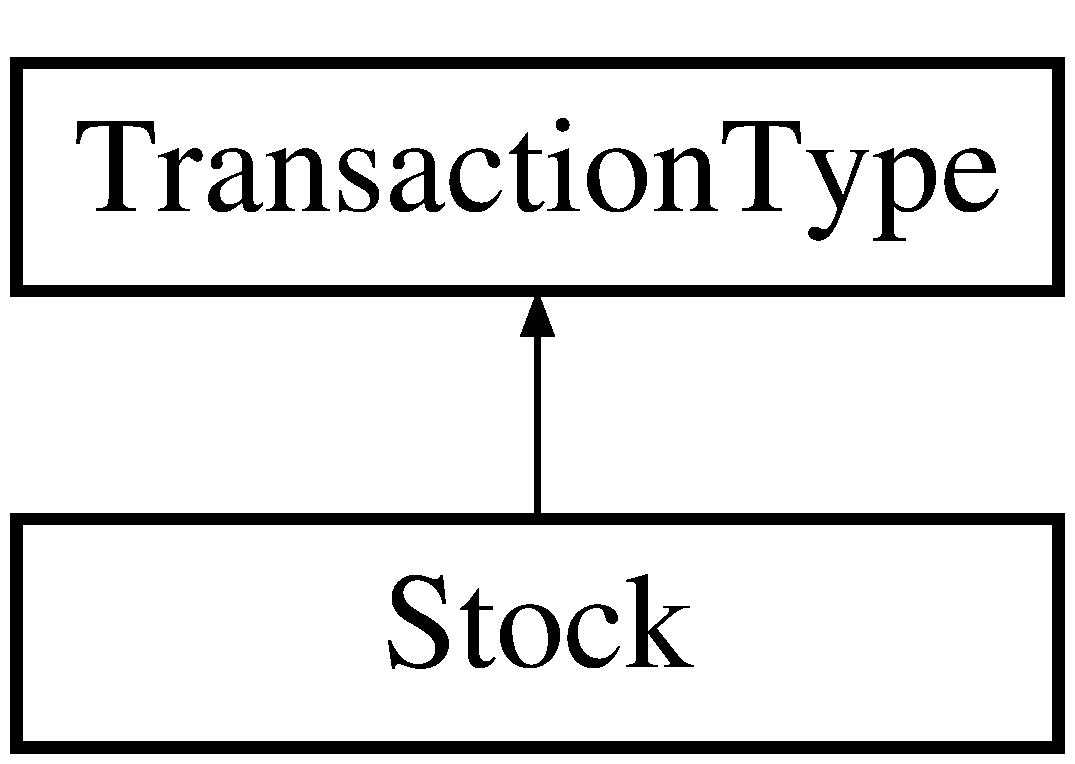
\includegraphics[height=2.000000cm]{class_stock}
\end{center}
\end{figure}
\subsection*{Public Member Functions}
\begin{DoxyCompactItemize}
\item 
\mbox{\Hypertarget{class_stock_adddc4282213b3174a4299cca5a30117c}\label{class_stock_adddc4282213b3174a4299cca5a30117c}} 
\mbox{\hyperlink{class_stock_adddc4282213b3174a4299cca5a30117c}{Stock}} ()
\begin{DoxyCompactList}\small\item\em Default Contrsuctor. \end{DoxyCompactList}\item 
\mbox{\Hypertarget{class_stock_a0527749d03379ba35706fcf48e7effa5}\label{class_stock_a0527749d03379ba35706fcf48e7effa5}} 
\mbox{\hyperlink{class_stock_a0527749d03379ba35706fcf48e7effa5}{Stock}} (std\+::string \mbox{\hyperlink{class_transaction_type_aad758d557417a18c944dc9849a390391}{ticker}}, int \mbox{\hyperlink{class_transaction_type_a079b40eebde548904529841f8746d4ff}{price}}, int \mbox{\hyperlink{class_transaction_type_a60b6221cf4b0bf30f5c4a4e15893b98d}{quantity}}, time\+\_\+t date)
\begin{DoxyCompactList}\small\item\em Parameter Constructor. \end{DoxyCompactList}\end{DoxyCompactItemize}
\subsection*{Additional Inherited Members}


The documentation for this class was generated from the following files\+:\begin{DoxyCompactItemize}
\item 
Backend/include/Stock.\+h\item 
Backend/src/Stock.\+cpp\end{DoxyCompactItemize}

\hypertarget{class_stock_csv_handler}{}\section{Stock\+Csv\+Handler Class Reference}
\label{class_stock_csv_handler}\index{Stock\+Csv\+Handler@{Stock\+Csv\+Handler}}


The \mbox{\hyperlink{class_stock_csv_handler}{Stock\+Csv\+Handler}} class.  




{\ttfamily \#include $<$Stock\+Csv\+Handler.\+h$>$}

\subsection*{Public Member Functions}
\begin{DoxyCompactItemize}
\item 
\mbox{\hyperlink{class_stock_csv_handler_a79a39d762f4dd87f82ee927c33f596cc}{Stock\+Csv\+Handler}} ()
\begin{DoxyCompactList}\small\item\em Constructor. \end{DoxyCompactList}\item 
\mbox{\hyperlink{class_stock_csv_handler_a9c197759533cc003c511d784a1cdb521}{$\sim$\+Stock\+Csv\+Handler}} ()
\begin{DoxyCompactList}\small\item\em Deconstructor. \end{DoxyCompactList}\item 
std\+::vector$<$ \mbox{\hyperlink{class_transaction_type}{Transaction\+Type}} $>$ \mbox{\hyperlink{class_stock_csv_handler_a3b32398ef8bf2994162802496d721333}{Import\+C\+SV}} ()
\begin{DoxyCompactList}\small\item\em Import C\+SV from input file path. \end{DoxyCompactList}\item 
bool \mbox{\hyperlink{class_stock_csv_handler_a5302fb4580cc69a73aa22a6e97e314ad}{Export\+C\+SV}} (std\+::vector$<$ \mbox{\hyperlink{class_transaction_type}{Transaction\+Type}} $>$ transactions)
\begin{DoxyCompactList}\small\item\em Export C\+SV to output file path. \end{DoxyCompactList}\item 
\mbox{\Hypertarget{class_stock_csv_handler_af0fa483a54671ac9cf6d14fb7991f3d3}\label{class_stock_csv_handler_af0fa483a54671ac9cf6d14fb7991f3d3}} 
void \mbox{\hyperlink{class_stock_csv_handler_af0fa483a54671ac9cf6d14fb7991f3d3}{set\+Input\+File\+Path}} (std\+::string path)
\begin{DoxyCompactList}\small\item\em Setter for input file path. \end{DoxyCompactList}\item 
\mbox{\Hypertarget{class_stock_csv_handler_a80849f00a57089ea30dde9947af3d4e3}\label{class_stock_csv_handler_a80849f00a57089ea30dde9947af3d4e3}} 
std\+::string \mbox{\hyperlink{class_stock_csv_handler_a80849f00a57089ea30dde9947af3d4e3}{get\+Input\+File\+Path}} ()
\begin{DoxyCompactList}\small\item\em Getter for input file path. \end{DoxyCompactList}\item 
\mbox{\Hypertarget{class_stock_csv_handler_a99b233b75f7039bfed3cc1a699af942c}\label{class_stock_csv_handler_a99b233b75f7039bfed3cc1a699af942c}} 
void \mbox{\hyperlink{class_stock_csv_handler_a99b233b75f7039bfed3cc1a699af942c}{set\+Output\+File\+Path}} (std\+::string path)
\begin{DoxyCompactList}\small\item\em Setter for output file path. \end{DoxyCompactList}\item 
\mbox{\Hypertarget{class_stock_csv_handler_aba4991b48238f173ecbe9b29ab850a0a}\label{class_stock_csv_handler_aba4991b48238f173ecbe9b29ab850a0a}} 
std\+::string \mbox{\hyperlink{class_stock_csv_handler_aba4991b48238f173ecbe9b29ab850a0a}{get\+Output\+File\+Path}} ()
\begin{DoxyCompactList}\small\item\em Getter for output file path. \end{DoxyCompactList}\end{DoxyCompactItemize}


\subsection{Detailed Description}
The \mbox{\hyperlink{class_stock_csv_handler}{Stock\+Csv\+Handler}} class. 

\subsection{Constructor \& Destructor Documentation}
\mbox{\Hypertarget{class_stock_csv_handler_a79a39d762f4dd87f82ee927c33f596cc}\label{class_stock_csv_handler_a79a39d762f4dd87f82ee927c33f596cc}} 
\index{Stock\+Csv\+Handler@{Stock\+Csv\+Handler}!Stock\+Csv\+Handler@{Stock\+Csv\+Handler}}
\index{Stock\+Csv\+Handler@{Stock\+Csv\+Handler}!Stock\+Csv\+Handler@{Stock\+Csv\+Handler}}
\subsubsection{\texorpdfstring{Stock\+Csv\+Handler()}{StockCsvHandler()}}
{\footnotesize\ttfamily Stock\+Csv\+Handler\+::\+Stock\+Csv\+Handler (\begin{DoxyParamCaption}{ }\end{DoxyParamCaption})}



Constructor. 

\mbox{\hyperlink{class_stock_csv_handler_a79a39d762f4dd87f82ee927c33f596cc}{Stock\+Csv\+Handler\+::\+Stock\+Csv\+Handler}}. \mbox{\Hypertarget{class_stock_csv_handler_a9c197759533cc003c511d784a1cdb521}\label{class_stock_csv_handler_a9c197759533cc003c511d784a1cdb521}} 
\index{Stock\+Csv\+Handler@{Stock\+Csv\+Handler}!````~Stock\+Csv\+Handler@{$\sim$\+Stock\+Csv\+Handler}}
\index{````~Stock\+Csv\+Handler@{$\sim$\+Stock\+Csv\+Handler}!Stock\+Csv\+Handler@{Stock\+Csv\+Handler}}
\subsubsection{\texorpdfstring{$\sim$\+Stock\+Csv\+Handler()}{~StockCsvHandler()}}
{\footnotesize\ttfamily Stock\+Csv\+Handler\+::$\sim$\+Stock\+Csv\+Handler (\begin{DoxyParamCaption}{ }\end{DoxyParamCaption})}



Deconstructor. 

\mbox{\hyperlink{class_stock_csv_handler_a9c197759533cc003c511d784a1cdb521}{Stock\+Csv\+Handler\+::$\sim$\+Stock\+Csv\+Handler}}. 

\subsection{Member Function Documentation}
\mbox{\Hypertarget{class_stock_csv_handler_a5302fb4580cc69a73aa22a6e97e314ad}\label{class_stock_csv_handler_a5302fb4580cc69a73aa22a6e97e314ad}} 
\index{Stock\+Csv\+Handler@{Stock\+Csv\+Handler}!Export\+C\+SV@{Export\+C\+SV}}
\index{Export\+C\+SV@{Export\+C\+SV}!Stock\+Csv\+Handler@{Stock\+Csv\+Handler}}
\subsubsection{\texorpdfstring{Export\+C\+S\+V()}{ExportCSV()}}
{\footnotesize\ttfamily bool Stock\+Csv\+Handler\+::\+Export\+C\+SV (\begin{DoxyParamCaption}\item[{std\+::vector$<$ \mbox{\hyperlink{class_transaction_type}{Transaction\+Type}} $>$}]{transactions }\end{DoxyParamCaption})}



Export C\+SV to output file path. 

\mbox{\hyperlink{class_stock_csv_handler_a5302fb4580cc69a73aa22a6e97e314ad}{Stock\+Csv\+Handler\+::\+Export\+C\+SV}}.


\begin{DoxyParams}{Parameters}
{\em transactions} & \\
\hline
\end{DoxyParams}
\begin{DoxyReturn}{Returns}

\end{DoxyReturn}
\mbox{\Hypertarget{class_stock_csv_handler_a3b32398ef8bf2994162802496d721333}\label{class_stock_csv_handler_a3b32398ef8bf2994162802496d721333}} 
\index{Stock\+Csv\+Handler@{Stock\+Csv\+Handler}!Import\+C\+SV@{Import\+C\+SV}}
\index{Import\+C\+SV@{Import\+C\+SV}!Stock\+Csv\+Handler@{Stock\+Csv\+Handler}}
\subsubsection{\texorpdfstring{Import\+C\+S\+V()}{ImportCSV()}}
{\footnotesize\ttfamily std\+::vector$<$ \mbox{\hyperlink{class_transaction_type}{Transaction\+Type}} $>$ Stock\+Csv\+Handler\+::\+Import\+C\+SV (\begin{DoxyParamCaption}{ }\end{DoxyParamCaption})}



Import C\+SV from input file path. 

\mbox{\hyperlink{class_stock_csv_handler_a3b32398ef8bf2994162802496d721333}{Stock\+Csv\+Handler\+::\+Import\+C\+SV}}.

\begin{DoxyReturn}{Returns}

\end{DoxyReturn}


The documentation for this class was generated from the following files\+:\begin{DoxyCompactItemize}
\item 
G\+U\+I/stock\+Tracker/Stock\+Csv\+Handler.\+h\item 
G\+U\+I/stock\+Tracker/Stock\+Csv\+Handler.\+cpp\end{DoxyCompactItemize}

\hypertarget{class_stock_model}{}\section{Stock\+Model Class Reference}
\label{class_stock_model}\index{Stock\+Model@{Stock\+Model}}
\subsection*{Public Member Functions}
\begin{DoxyCompactItemize}
\item 
\mbox{\Hypertarget{class_stock_model_aa5de5466e50f2bba375387dd35158b9d}\label{class_stock_model_aa5de5466e50f2bba375387dd35158b9d}} 
bool {\bfseries Add\+Transaction} (std\+::string symbol, int quantity, int price, \mbox{\hyperlink{class_transaction_type}{Transaction\+Type}} type)
\item 
\mbox{\Hypertarget{class_stock_model_a2ace2720dc1742b8d563b96bb2e81eec}\label{class_stock_model_a2ace2720dc1742b8d563b96bb2e81eec}} 
bool {\bfseries Remove\+Transaction} (std\+::string symbol, int quantity, int price, \mbox{\hyperlink{class_transaction_type}{Transaction\+Type}} type)
\item 
\mbox{\Hypertarget{class_stock_model_afcd1e771bc7417eb735ab383d24d4988}\label{class_stock_model_afcd1e771bc7417eb735ab383d24d4988}} 
std\+::vector$<$ \mbox{\hyperlink{class_transaction_type}{Transaction\+Type}} $>$ {\bfseries Get\+Transactions} (std\+::string symbol)
\item 
\mbox{\Hypertarget{class_stock_model_ac892a9e35bc731342d92c84f5e0bfff6}\label{class_stock_model_ac892a9e35bc731342d92c84f5e0bfff6}} 
\mbox{\hyperlink{class_transaction_type}{Transaction\+Type}} {\bfseries Get\+Stock\+Data} (std\+::string symbol)
\item 
\mbox{\Hypertarget{class_stock_model_af9ac92e3e10b39f999ea5a41a96b7b9c}\label{class_stock_model_af9ac92e3e10b39f999ea5a41a96b7b9c}} 
int {\bfseries Calculate\+Performance} ()
\end{DoxyCompactItemize}


The documentation for this class was generated from the following files\+:\begin{DoxyCompactItemize}
\item 
Backend/include/Stock\+Model.\+h\item 
Backend/src/Stock\+Model.\+cpp\end{DoxyCompactItemize}

\hypertarget{class_transaction_type}{}\section{Transaction\+Type Class Reference}
\label{class_transaction_type}\index{Transaction\+Type@{Transaction\+Type}}


The \mbox{\hyperlink{class_transaction_type}{Transaction\+Type}} class is a base class for sub types.  




{\ttfamily \#include $<$Transaction\+Type.\+h$>$}

Inheritance diagram for Transaction\+Type\+:\begin{figure}[H]
\begin{center}
\leavevmode
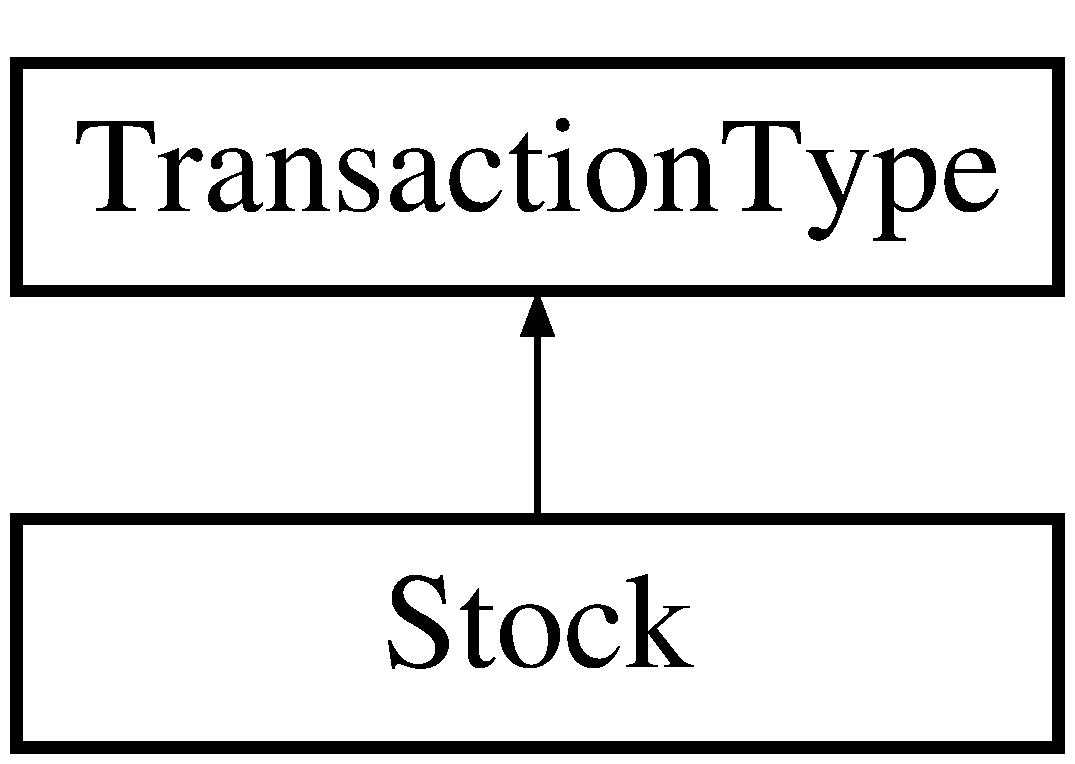
\includegraphics[height=2.000000cm]{class_transaction_type}
\end{center}
\end{figure}
\subsection*{Public Member Functions}
\begin{DoxyCompactItemize}
\item 
\mbox{\Hypertarget{class_transaction_type_af74ebcedbda4d46f90de333b9268b8a8}\label{class_transaction_type_af74ebcedbda4d46f90de333b9268b8a8}} 
\mbox{\hyperlink{class_transaction_type_af74ebcedbda4d46f90de333b9268b8a8}{Transaction\+Type}} ()
\begin{DoxyCompactList}\small\item\em Default constructor. \end{DoxyCompactList}\item 
\mbox{\Hypertarget{class_transaction_type_a0600069544b2650a1cbd3b4f99d80c8a}\label{class_transaction_type_a0600069544b2650a1cbd3b4f99d80c8a}} 
int \mbox{\hyperlink{class_transaction_type_a0600069544b2650a1cbd3b4f99d80c8a}{Check\+Equals}} (\mbox{\hyperlink{class_transaction_type}{Transaction\+Type}} other)
\begin{DoxyCompactList}\small\item\em Compares two \mbox{\hyperlink{class_transaction_type}{Transaction\+Type}} objects. \end{DoxyCompactList}\item 
std\+::string \mbox{\hyperlink{class_transaction_type_ae93afca932014b0dfa4d1a3a66ca0ad2}{To\+C\+SV}} ()
\begin{DoxyCompactList}\small\item\em Formats the object for csv export. \end{DoxyCompactList}\item 
\mbox{\Hypertarget{class_transaction_type_ac139f76c5ae460bd9c1c87570c6bee34}\label{class_transaction_type_ac139f76c5ae460bd9c1c87570c6bee34}} 
int \mbox{\hyperlink{class_transaction_type_ac139f76c5ae460bd9c1c87570c6bee34}{Get\+Price}} ()
\begin{DoxyCompactList}\small\item\em Getter for the price. \end{DoxyCompactList}\item 
\mbox{\Hypertarget{class_transaction_type_aecf32eadd4975d6284bcc031c8624daf}\label{class_transaction_type_aecf32eadd4975d6284bcc031c8624daf}} 
void \mbox{\hyperlink{class_transaction_type_aecf32eadd4975d6284bcc031c8624daf}{Set\+Price}} (int \mbox{\hyperlink{class_transaction_type_a079b40eebde548904529841f8746d4ff}{price}})
\begin{DoxyCompactList}\small\item\em Setter for the price. \end{DoxyCompactList}\item 
\mbox{\Hypertarget{class_transaction_type_a2b81258ca5237f8c07e2bdd43f0ffde1}\label{class_transaction_type_a2b81258ca5237f8c07e2bdd43f0ffde1}} 
int \mbox{\hyperlink{class_transaction_type_a2b81258ca5237f8c07e2bdd43f0ffde1}{Get\+Quantity}} ()
\begin{DoxyCompactList}\small\item\em Getter for the quantity. \end{DoxyCompactList}\item 
\mbox{\Hypertarget{class_transaction_type_a3fda2989a38f1564e7761cc26bbfc8ca}\label{class_transaction_type_a3fda2989a38f1564e7761cc26bbfc8ca}} 
void \mbox{\hyperlink{class_transaction_type_a3fda2989a38f1564e7761cc26bbfc8ca}{Set\+Quantity}} (int \mbox{\hyperlink{class_transaction_type_a60b6221cf4b0bf30f5c4a4e15893b98d}{quantity}})
\begin{DoxyCompactList}\small\item\em Setter for the qunatity. \end{DoxyCompactList}\item 
\mbox{\Hypertarget{class_transaction_type_a88fd57a09996e67178256cd8e76cb3e4}\label{class_transaction_type_a88fd57a09996e67178256cd8e76cb3e4}} 
std\+::string \mbox{\hyperlink{class_transaction_type_a88fd57a09996e67178256cd8e76cb3e4}{Get\+Ticker}} ()
\begin{DoxyCompactList}\small\item\em Getter for the ticker. \end{DoxyCompactList}\item 
\mbox{\Hypertarget{class_transaction_type_a7210ad6704fa3b65d440dd46fe1044e2}\label{class_transaction_type_a7210ad6704fa3b65d440dd46fe1044e2}} 
void \mbox{\hyperlink{class_transaction_type_a7210ad6704fa3b65d440dd46fe1044e2}{Set\+Ticker}} (std\+::string \&\mbox{\hyperlink{class_transaction_type_aad758d557417a18c944dc9849a390391}{ticker}})
\begin{DoxyCompactList}\small\item\em Setter for the ticker. \end{DoxyCompactList}\item 
\mbox{\Hypertarget{class_transaction_type_a5e4e3170dda80d69f67efd3044bb30e0}\label{class_transaction_type_a5e4e3170dda80d69f67efd3044bb30e0}} 
time\+\_\+t \mbox{\hyperlink{class_transaction_type_a5e4e3170dda80d69f67efd3044bb30e0}{Get\+Date}} ()
\begin{DoxyCompactList}\small\item\em Getter for the date. \end{DoxyCompactList}\item 
\mbox{\Hypertarget{class_transaction_type_aefd70a5b3d72944d0ddd7aa289c0021a}\label{class_transaction_type_aefd70a5b3d72944d0ddd7aa289c0021a}} 
void \mbox{\hyperlink{class_transaction_type_aefd70a5b3d72944d0ddd7aa289c0021a}{Set\+Date}} (time\+\_\+t date)
\begin{DoxyCompactList}\small\item\em Setter for the date. \end{DoxyCompactList}\end{DoxyCompactItemize}
\subsection*{Protected Attributes}
\begin{DoxyCompactItemize}
\item 
\mbox{\Hypertarget{class_transaction_type_a079b40eebde548904529841f8746d4ff}\label{class_transaction_type_a079b40eebde548904529841f8746d4ff}} 
int \mbox{\hyperlink{class_transaction_type_a079b40eebde548904529841f8746d4ff}{price}}
\begin{DoxyCompactList}\small\item\em Integer to store the price of stock at transaction. \end{DoxyCompactList}\item 
\mbox{\Hypertarget{class_transaction_type_a60b6221cf4b0bf30f5c4a4e15893b98d}\label{class_transaction_type_a60b6221cf4b0bf30f5c4a4e15893b98d}} 
int \mbox{\hyperlink{class_transaction_type_a60b6221cf4b0bf30f5c4a4e15893b98d}{quantity}}
\begin{DoxyCompactList}\small\item\em Integer to store the quantity of stock in transaction. \end{DoxyCompactList}\item 
\mbox{\Hypertarget{class_transaction_type_aad758d557417a18c944dc9849a390391}\label{class_transaction_type_aad758d557417a18c944dc9849a390391}} 
std\+::string \mbox{\hyperlink{class_transaction_type_aad758d557417a18c944dc9849a390391}{ticker}}
\begin{DoxyCompactList}\small\item\em String to store ticker symbol. \end{DoxyCompactList}\item 
\mbox{\Hypertarget{class_transaction_type_afb98c9a6a95e2fd8157448edb9eeecce}\label{class_transaction_type_afb98c9a6a95e2fd8157448edb9eeecce}} 
time\+\_\+t {\bfseries date}
\end{DoxyCompactItemize}


\subsection{Detailed Description}
The \mbox{\hyperlink{class_transaction_type}{Transaction\+Type}} class is a base class for sub types. 

\subsection{Member Function Documentation}
\mbox{\Hypertarget{class_transaction_type_ae93afca932014b0dfa4d1a3a66ca0ad2}\label{class_transaction_type_ae93afca932014b0dfa4d1a3a66ca0ad2}} 
\index{Transaction\+Type@{Transaction\+Type}!To\+C\+SV@{To\+C\+SV}}
\index{To\+C\+SV@{To\+C\+SV}!Transaction\+Type@{Transaction\+Type}}
\subsubsection{\texorpdfstring{To\+C\+S\+V()}{ToCSV()}}
{\footnotesize\ttfamily std\+::string Transaction\+Type\+::\+To\+C\+SV (\begin{DoxyParamCaption}{ }\end{DoxyParamCaption})}



Formats the object for csv export. 

This method outputs the object to a C\+SV format Returns a string with the values comma delimited 

The documentation for this class was generated from the following files\+:\begin{DoxyCompactItemize}
\item 
Backend/include/Transaction\+Type.\+h\item 
Backend/src/Transaction\+Type.\+cpp\end{DoxyCompactItemize}

%--- End generated contents ---

% Index
\backmatter
\newpage
\phantomsection
\clearemptydoublepage
\addcontentsline{toc}{chapter}{Index}
\printindex

\end{document}
